\section{Classification}
The classification is the main target for the proof-of-concept 
implementation, described below. 

The main targets for the classification algorithm is determined by some 
spatial clustering algorithm. This data set might either be entire 
Moments if no cluster is found, or if the entire data set is regarded to
be a cluster. If several clusters are found, these will be classified 
individually. Moments or clusters sent to the classification algorithm 
will below be referenced to as an activity (not to be confused with the
later mentioned class \emph{activity}, representing the amount of
physical activity).

\subsection{Input Beliefs - Evidence}
%%%%%%%%%%%%%%%%%%%%%%%%%%%%%%%%%%%%%%%%%%%% 80 line marker %%%%%%%%%%%%%%%
In order to establish a prior belief in the data to model, it is 
necessary to model the estimated prior distribution of the input data to 
model the prior belief in class assignment. This is later updated based on 
observations of the data, and beliefs are reinforced or skewed based on 
these observations into \emph{posterior beliefs}.

\subsubsection{Accelerometer}
The accelerometer provides 3 values for each sample taken by the sensor, 
one for each direction in the three dimensional coordinate system. As the 
Clip can be mounted on the user in different ways, as well as being tilted, 
these acceleration vectors are not bound to some specific orientation in
relation with the earths coordinate system.

Most commonly the Clip is either fitted on the user with the buckle facing
down, or horizontally (either left or right). This makes the x-axis and
y-axis interchangeable.

\begin{figure}[ht]
    \centering
    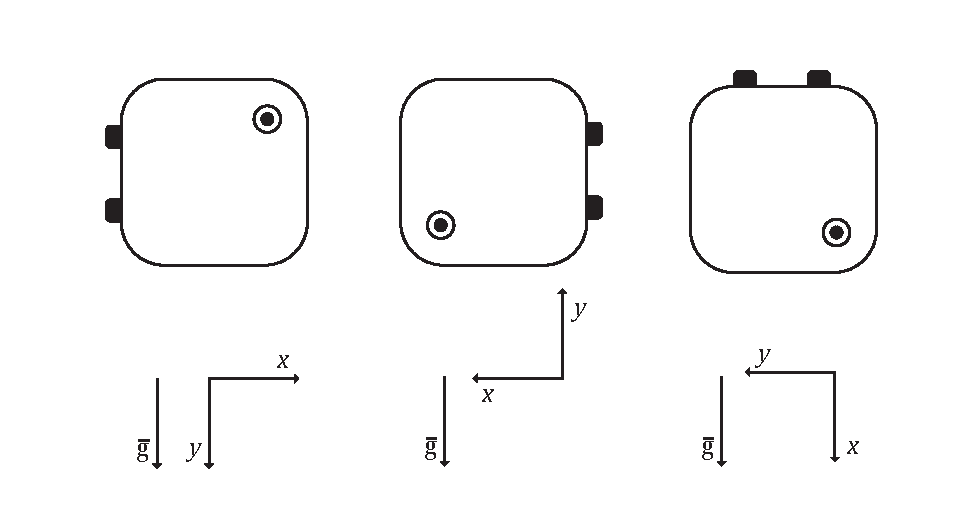
\includegraphics[width=0.7\textwidth]{images/narrative_clip_orientation.pdf}
    \caption{ An illustration of the most plausible orientations of The Clip as 
        worn by the user. \label{fig:narrative-clip-orientation} }
\end{figure}

Given the uncertainty of which direction the sample was recorded in, the
solution would be to use the magnitude of the vectors combined, and 
ignore the direction of the resulting vector\footnote{
    If the Clips orientation was of interest, or there was a specific need
    to know each composant of the accelerometer vector, it could be assumed
    that the composant being closest to $ g \approx 9.8 m/s^2 $ in magnitude was 
    the direction facing downward. The user is not likely to change the 
    orientation of the Clip between each photo, so detecting the orientation
    based on multiple photos seems more robust and feasible. 
}. Chances that the combined
vectors should sum up to the original, stationary vector when moving seem
slim. 

An accelerometer measures \emph{proper acceleration}\footnote{
    Proper acceleration is the physical acceleration that is experienced 
    by an object, including gravitational force. }
and will therefore usually have a constant approximated value corresponding 
to $ g \approx 9.8 m/s^2 $ when stationary, and somewhere around that value when
a user is in motion. 

The most feasible application of the accelerometer seems to be determining
the level of activity in the Moment. When a user is active (such as being
out for a run or sporting), it is probable that the acceleration is varying, 
partly because of the actual movement, and partly because the Clip jiggles 
around when in movement. 

Given the above, the most feasible distribution of the samples observed
seem to be around $g$, with decreasing probability around this point as
the acceleration diverges more and more from $g$. Such a distribution
could be described using a 
\emph{Normal distribution} with the following \emph{probability density 
function}:
\begin{definition}[Normal Distribution Probability Density Function]
\label{definition:normal-pdf}
$$
    PDF_{Norm}(x, \mu, \sigma) = 
        \frac{1}{\sigma \sqrt{2\pi} } 
                 e^{ -\frac{(x-\mu)^2}{2\sigma^2} }
$$
\end{definition}

We denote a stochastic variable that is Normally distributed by
\begin{definition}[Normally distributed variable]
\label{definition:normal-variable}
$$
    X_i \sim Norm(\mu, \sigma)
$$
\end{definition}
where $\mu$ is the expected mean value (which we expect to be $g \approx 9.8 m/s^2$
or equivalent), and $\sigma$ the standard deviation.

In order to measure how the acceleration varies, the 
\emph{auto-correlation} (or serial correlation) of the samples can be used. The 
auto-correlation is defined as the cross-correlation of a series of 
samples with itself. This is generally used in statistics as a measurement of 
the predictability of a series of samples from a distribution, and predicts 
how much a value is likely to change given two consecutive measurements. 

This is another reason to use the magnitude of the accelerometer vector, as
values close to 0 (as the y- and z-axis tend to be while stationary) show 
very little auto-correlation, due to small changes in small values.

\subsubsection{Area}
The area size of an activity. When there are no spatial data points
available for an activity, this is for simplicity reasons assumed to 
be $0$, indicating that a user is in such a small area that it can be
neglected. 
\begin{definition}[Area distribution]
\label{definition:area-variable}
$$
    X_{area} \sim Norm(\mu_{area}, \sigma_{area})
$$
\end{definition}
where $\mu_{area}$ is found by using the mean area value in a subset of 
all currently sampled activities, and $\sigma$ is the variance in the same 
data set.  

\subsubsection{Face Detection}
Narrative runs a face detection algorithm on the set of their images, 
determining whether any face is present or not in a photo. The ratio 
between images with faces and without are of particular interest, as we can 
see below, and is deduced for each activity in the classification algorithm. 
The faces/photos distribution is modelled as 
\begin{definition}[Faces/Photos distribution]
\label{definition:faces-variable}
$$
    X_{faces} \sim Norm(\mu_{faces}, \sigma_{faces})
$$
\end{definition}
where $\mu$ is found by using the mean value in a subset of all currently 
stored activities, and $\sigma$ is the variance in the same data set.  

\subsubsection{Time}
The starting time of a Moment is probably more likely to occur mid-day or 
during the evening, when more special activities occur and the users decide 
to clip it on. This timely information is used to detect where users are 
spending their time, and if their activity is work-related or recreational, 
on their spare time. The probability of observing such a timestamp is therefor 
estimated using a \emph{Binomial Distribution}, with the following
\emph{probability mass function}\footnote{
    This is denoted \emph{probability mass function} instead of the 
    previously mentioned \emph{probability density function}. This is 
    essentially the same thing, with the difference of the first being
    a continuous distribution while the latter is discrete. }:
\begin{definition}[Binomial Distribution Probability Mass Function]
\label{definition:binomial-pmf}
$$
    PMF_{Bin}(k;n, p) = \Pr(X = k) = {n\choose k}p^k(1-p)^{n-k}
$$
\end{definition}

We denote a stochastic variable that is Binomially distributed by
\begin{definition}[Binomially distributed variable]
\label{definition:binomial-variable}
$$
    X_i \sim Bin(n, p)
$$
\end{definition}
where $n$ is the number of trials attempted and $p$ is the expected
number of successes.

\subsection{Output Beliefs}
The target is to classify a received data set into a finite set of classes. 
According to Bayesian methodology, it is necessary to model an experts 
belief in the distribution of assigned classes. First of all, assume that 
an input data set can never partly be assigned a class but always fully. 
The assignment is either done, or not. This model was described by the 
Swiss mathematician Jakob Bernoulli, who coined the 
\emph{Bernoulli distribution} with the following probability mass function:
\begin{definition}[Bernoulli Probability Mass Function]
\label{definition:bernoulli-pmf}
$$
    PMF_{Bernoulli}(k,p) =
    \begin{cases} 
        p   & \mathrm{if} \; k = 1 \\
        1-p & \mathrm{if} \; k = 0 \\
    \end{cases}
$$
\end{definition}
This describes the probability $p$ of a class being assigned to the data 
set received. We denote a stochastic variable that is Bernoulli 
distributed, the prior probability of a class $i$ being assigned, by
\begin{definition}[Bernoulli distributed variable]
\label{definition:bernoulli-variable}
$$
    X_i \sim Ber(p_i)
$$
\end{definition}

This prior probability is modelled by one or several threshold values,
which determine the probability of which class is used. 

The inferred classes that we will attempt to predict are the following:
\begin{itemize}
    \item \emph{Social} - Whether the user is engaging in a social 
        activity or not. This is believed to be effected by the amount
        of faces in the photos in a series. 
    \item \emph{Working} - The users working status during a Moment. 
        This is believed to be affected by the starting point of the 
        series of images, as well as the area size of the detected
        clusters. 
    \item \emph{Indoors} - Whether the user is indoors or not. This is 
        believed to be affected by the area size of an activity.
    \item \emph{Movement} - How much physical activity the user is 
        undergoing during an activity. This is 
        believed to be affected by the auto-correlations mean value 
        of an activity.
\end{itemize}

These classes can take on two discrete values; either they are assigned
or not (this is somewhat simplified with the labels for the classes - 
with friends or not alone, for \emph{Social}, working or off hours
for \emph{Working} and indoors or outdoors for \emph{Indoors}). Thus, 
these are Bernoulli distributed as mentioned above:
\begin{equation}
    \label{eq:bernoulli-classification}
    \begin{split}
        X_{social}  &\sim Ber(p_{social})  \\
        X_{indoors} &\sim Ber(p_{indoors}) \\
        X_{working} &\sim Ber(p_{working}) 
    \end{split}
\end{equation}
where $p_i$ depends on the parent values (see 
figure~\ref{fig:bayes-network} on page~\pageref{fig:bayes-network}).

The exception here is $X_{activity}$ which is 
\emph{Categorically distributed}, a generalization of the Bernoulli
distribution:
\begin{definition}[Categorical Probability Mass Function]
\label{definition:categorical-pmf}
$$
    PMF_{Categorical}(k,p) = p_i
$$
\end{definition}
where $p_i$ represents the probability case $i$ to be true. 
We denote a stochastic variable that is Categorically 
distributed, the prior probability of a class $i$ being assigned, by
\begin{definition}[Categorically distributed variable]
\label{definition:categorical-variable}
$$
    X_i \sim Cat(p_1, ..., p_i)
$$
\end{definition}

It is worth reminding here that it is the concept of using Bayesian 
Inference as a classification tool for life-logging environments that 
is up for testing, and not necessarily the model for each 
implementation. As mentioned among the limitations, the structure of
the network is assumed to be fixed from the start and automated learning
of the structure is not applicable. 
Because of this, it seems more suitable to infer a rather 
simple and shallow model to test the concept. Using several classes
that only depend on a few parameters allow some error and redundancy 
to sneak in due to model construction errors, which will be discussed 
later in this thesis.  

\subsection{Model Parameters}
All parameters mentioned above can be observed by inspecting data, and 
are thus the evidence $E$ that can be observed when the model is in certain 
world state. Modelling these correctly is nevertheless important anyway, in 
the case of missing values. 

The classification depends on a series of model parameters, such as thresholds
for when different classes should be inferred. 

These breakpoints are be denoted as model parameters, and are of interest for
learning how classification can be done. While approximating these with a 
well-formed probability function is a cause for faster convergence and faster
learning, it is essential that all possibilities are covered. If the model 
parameter is not covered by it's initial probabilities, the model is not 
correct and will probably not provide the desired results. 

These model parameters will for simplicity's sake be universal in this master
thesis, but should probably later on be possible to tweak for each individual, 
with the aid of a learned starting point.

\subsubsection{Learning the parameters}
In order to make our hypothesis as credible as possible given previously 
recorded classifications made by human observation, the thresholds need to
be properly set. This is done by letting both our samples of the observed
data of several Moments be fixed, as well as the classification that later
is to be determined for other activities. The only thing that is then allowed
to vary in order to make the model true, is the thresholds, our hypothesis, 
forcing these variables to take on relevant values. 

By doing this for a decent amount of pre-determined classifications, 
and letting MCMC in PyMC fit the model by drawing thousands of samples of this 
distribution, by randomly walking over the set, something very close to the 
true distribution is learned, that can be used as the hypothesis in future 
classifications. 

In this instance, a rather small sample is used, yielding a hypothesis 
in danger of being biased. In a real-world application, this sample of
classification would be much bigger, but this sample size of ~50 classifications
should suffice to prove the concept. 

\subsection{The Bayesian Network}
The dependencies between various stochastic variables can be made more 
over-viewable when represented graphically as a network, see 
figure~\ref{fig:bayes-network}. In this figure, the top ellipsoids with a solid 
border marks the evidence $E$ observed for each activity. The squares are the 
thresholds, or model parameters that have been learnt via Bayesian inference
and fitting the model with pre-classified data. This is our hypothesis. 
The circles with a dashed border is the classes of which we try to determine 
our posterior belief after observing the evidence.

\begin{figure}[ht]
    \centering
    \includegraphics[width=0.8\textwidth]{images/bayes_network.pdf}
    \caption{A graphical view of the bayesian network modelled for deriving the
        classes. \label{fig:bayes-network} }
\end{figure}

\subsection{Curse of Dimensionality}
The \emph{curse of dimensionality} is a problem that arises in cluster 
analysis and data mining applications where a lot of dimensions or 
considered features in the regarded data causes data that are fairly 
similar to appear to be very dissimilar due a few to outlying, less 
important property values. 

This problem arises when the observed data contains a lot of parameters that 
can take on very different values.

In this work, this is mainly a problem in the inference domain and not in the 
spatial clustering domain, as spatial data in 
it's nature is two-dimensional (at least in this case, as the earths
surface can be regarded as two-dimensional, from a geographical point of 
view).

This is why clustering of spatial points precedes the Bayesian inference 
in this work, in order of decreasing the dimensionality and learning 
something useful from the spatial data before moving on to tackle other 
quantifiable data: as for each comparable spatial point in the data set, we 
would need to model some sort of random variable, mapping against one 
dimension. This could easily sum up to several hundreds of dimensions, in 
the spatial analysis alone! Clustering algorithms exist in Bayesian 
notations as well, and one might even attempt to formulate the ones 
mentioned in this report in a more statistical-oriented fashion, but the 
main advantage here is to decrease the number of dimensions for further 
analysis in several steps. A pitfall to watch out for with this approach 
is removing more information than necessary, and thus making a biased 
analysis at a later stage due to unintentional biased information loss.

\subsection{Evaluating the Classification}
The proof-of-concept implementation will double as an evaluation program
visualizing users Moments and providing the deducted classifications, and
at the same time receive feedback from the users.

This is implemented as a browser extension, adding content to Narratives
web application and allows users to get classifications provided by the 
Bayesian inference framework set up for their own Moments. This as no one 
knows better how to classify an activity than the user who performed it, 
and therefore no one should be better at evaluating the algorithm 
performing classifications on it. 

Firstly, the users are presented with the option to run the classification
algorithm on a Moment (as they might choose not to provide every Moment
for the study for privacy purposes). When choosing to classify, a
visually comprehensive overview of their images and whereabouts during
this Moment is presented to them, as well as a classification of the 
activity or activities. After this, the users are provided with a form
where they evaluate the classifications quality on a 5-step scale, as
well as perform the same classification as the algorithm did. A comment
field is also present for commenting on the classification performance. 

In this scenario, in order to evaluate the algorithms performance, the 
users classifications is regarded as the truth. Some error can of course
be introduced in the form of users misinterpreting class definitions, but
this will be assumed to be an negligible amount of error.

Weighed into this is also the amount of false positives and false negatives
encountered. A false positive is considered to be a wrongful classification
where a \emph{semantically charged} class is chosen over a more neutral class, 
whereas a false negative denotes the opposite. These semantically charged
classes consists of the a set of classes that would actually be visible to 
the end user in a real implementation, since these denotes that something 
special happening in an activity, and considered more interesting than the
alternative. An example of this being that the social label 
\emph{With Friends} is probably more interesting and attractive to the user 
than the alternative \emph{Alone}. A false positive would in this case 
be for an algorithm to select a label \emph{With Friends} for a users
activity when the user actually was alone. 

\section{Clustering}

Three algorithms are chosen for evaluating various algorithms for clustering, 
each being a representative from the traditional breakdown of clustering 
algorithm types\footnote{
    For a more precise overview of these algorithms than provided in the
    previous chapter, please see 
    appendix~\ref{app:clustering-algorithms-theory}. }:
\begin{itemize}
    \item CLARANS
    \item DBSCAN
    \item SLINK
\end{itemize}

Because clustering algorithms differ very much, both in execution but also in 
output, these will be assessed in slightly different ways. The algorithms are
tested on the same data sets and output will be compared both by using 
silhouettes and run-time, but also evaluated by the extra features that each 
algorithm bring. In the end, the suitability for this particular task of 
detecting clusters in data sets on the move is evaluated, and anything an 
algorithm can provide as an advantage will be taken into account. The results
of the silhouettes and run-time will be presented in the following chapter,
while the latter discussion of further algorithm advantages will be discussed
in the discussion chapter. 

\subsection{Clustering parameters}
When using clustering algorithms, the cluster parameters are important tools 
for describing what type of clusters that are desired. Therefore, some 
guidelines are introduced as to how the cluster parameters are set when 
evaluating the cluster performance of the algorithms.

\subsubsection{CLARANS}
CLARANS runs several times over the data set, with different $k$. Inspection
shows that these data sets seldom contains more than a few clusters, so therefore
$k$ will go from 1 to 5 in order of finding a suitable $k_{nat}$\footnote{
    In the original report, CLARANS is meant to throw away clusters producing
    clusters with no significant structure found. This is its way of disregarding
    noise. It is not done in this thesis, as for potential detection of 
    activities, these clusters would be used as travels from one activity to
    another. }.

As for $num\_local$ and $max\_neighbour$, these need to be large enough that
it is likely that a good solution is found. Setting these to $10\%$ and 
$20\%$ of the desired data set respectively, seems to lead to consistent results. 

\subsubsection{DBSCAN}
A main upside of DBSCAN is its ability to discard points as noise, 
which proves useful in this particular case where combinations of 
clusters and paths exists, and paths can be discarded by tweaking 
the clustering parameters $ \epsilon $ and $ minPts $. This is the case
when we want to discard paths for instance walking speed, $ v_{walking} $
if we choose  $ \epsilon $ and $ minPts $ as 
\begin{equation}
    \label{eq:minPts_eps_condition}
    minPts \times v_{walking} \times 30 < \epsilon - C_{margin}
\end{equation}
with some safety margin constant $ C_{margin} $. This condition is 
illustrated in figure~\ref{fig:epsilon_minpts_condition}.

\begin{figure}[ht]
    \centering
    \includegraphics[width=0.5\textwidth]{images/epsilon_minpts_condition.pdf}
    \caption{ An illustration of the condition for choosing $ \epsilon $ and 
              $ minPts $ to exclude paths. \label{fig:epsilon_minpts_condition} }
\end{figure}

In order of keeping clusters significant enough, we let $minPts$ be
$10\%$ of the size of the data set, and set $C_{margin}$ to 
$minPts \times v_{walking} \times 15$, and let $\epsilon$ take
on the smallest value possible while still fulfilling 
equation~\ref{eq:minPts_eps_condition}.

\subsubsection{SLINK}
SLINK's cutoff function will consist of a distance cutoff condition same as 
DBSCAN's $ \epsilon $. 

\subsection{Detected Clusters}
A frequent scenario for using the Clip is when the user puts it on, then 
carries around for a long period of time at several locations, experiencing 
different activities. Deduction of qualitative information from life-logging 
experiences revolve partially around distinguishing these activities from 
each other, and this is where spatial clustering comes in handy. In this 
particular instance, a form of clustering has already been done, partitioning
long series of images into Moments using timestamps and RGB-cubes from photos
to detect the start of a new Moment. 

Therefore it is preferable to run the proposed spatial clustering algorithms
earlier in the pipeline than the proof-of-concept implementation in this paper
suggests, and this is why these algorithms will be tested on data sets not
only consisting of said Moments. But, as stated above, the proof-of-concept
implementation will only contain spatial clustering on a Moment-level. This 
will be provided by DBSCAN, as it is better suited for small data-sets where
only one cluster is found, or none at all for that matter. The algorithm
comparison however, will run on bigger data sets. 

A distinction between when a cluster has been detected and not has to be made 
as well, as the absence of a cluster can be interpreted as a user travelling 
between two sites.

\subsection{Assessed Spatial Data Sets}
The data sets on which the algorithms performance is assessed are real-world
spatial GPS data from users, chosen in a representative manner. The sets 
displayed in this report do not contain any map background, in order to
preserve anonymity.

These data sets consist both of data already divided into Moments, and 
longer data series merged together, providing more quantitative clustering
possibilities, and more possible clusters. 

\section{Big Data Ethics}
Given the current development of the technology revolving around Big Data
and deducting user behaviour given statistical information where the privacy 
of the end users needs to be discussed. Current literature and articles are
evaluated to get an overview of the current status of the debate, with 
the focus of life-logging devices as company services. 
